\section{Motivation}

\normalsize
\subsection{Lake Michigan Tributaries Inclusion}

EPA has started a modeling program for determining the best strategy to manage toxic chemicals control. The chemicals included in the program are PCBs, trans-nonachlor, atrazine, and mercury. To model the transport, fate and bioaccumulation of those chemicals, the model includes a hydrodynamic submodel to estimate the velocity field, temperature field, bottom shear stress, turbulence parameters, free surface level, and wind wave interaction; these estimates are then used to simulate sediment transport, water quality, and toxic transport in other submodels. This hydrodynamic submodel was modified by Schwab, et al. \cite{SCHWAB1994, SCHWAB1998} from a three-dimensional ocean circulation model which was first developed at Princeton University by Blumberg and Mellor \cite{Blumberg1987}. However, this Lake Michigan hydrodynamic model has several weaknesses \cite{SCHWAB1998}: (1) the lack of an ice model causes significant violation of the lake's heat balance during the winter. As a result, the model fails to predict the temperature field correctly; (2) the exclusion of tributaries and outflow through the Straits of Mackinac violates the mass balance over a long period of time; (3) the lack of adequate horizontal resolution hinders the model's ability to describe the observed currents sufficiently, resolve baroclinic motion in summer adequately, and simulate the thermocline without diffusivity.

The numerical simulation of Lake Michigan with the inclusion of tributaries and the connection with Lake Huron has motivated researches such as the receding boundary method for domain decomposition, and the adjustable non-hydrostatics method as an alternative treatment for the incompressible assumptions.

\begin{figure}[h]
\begin{center}
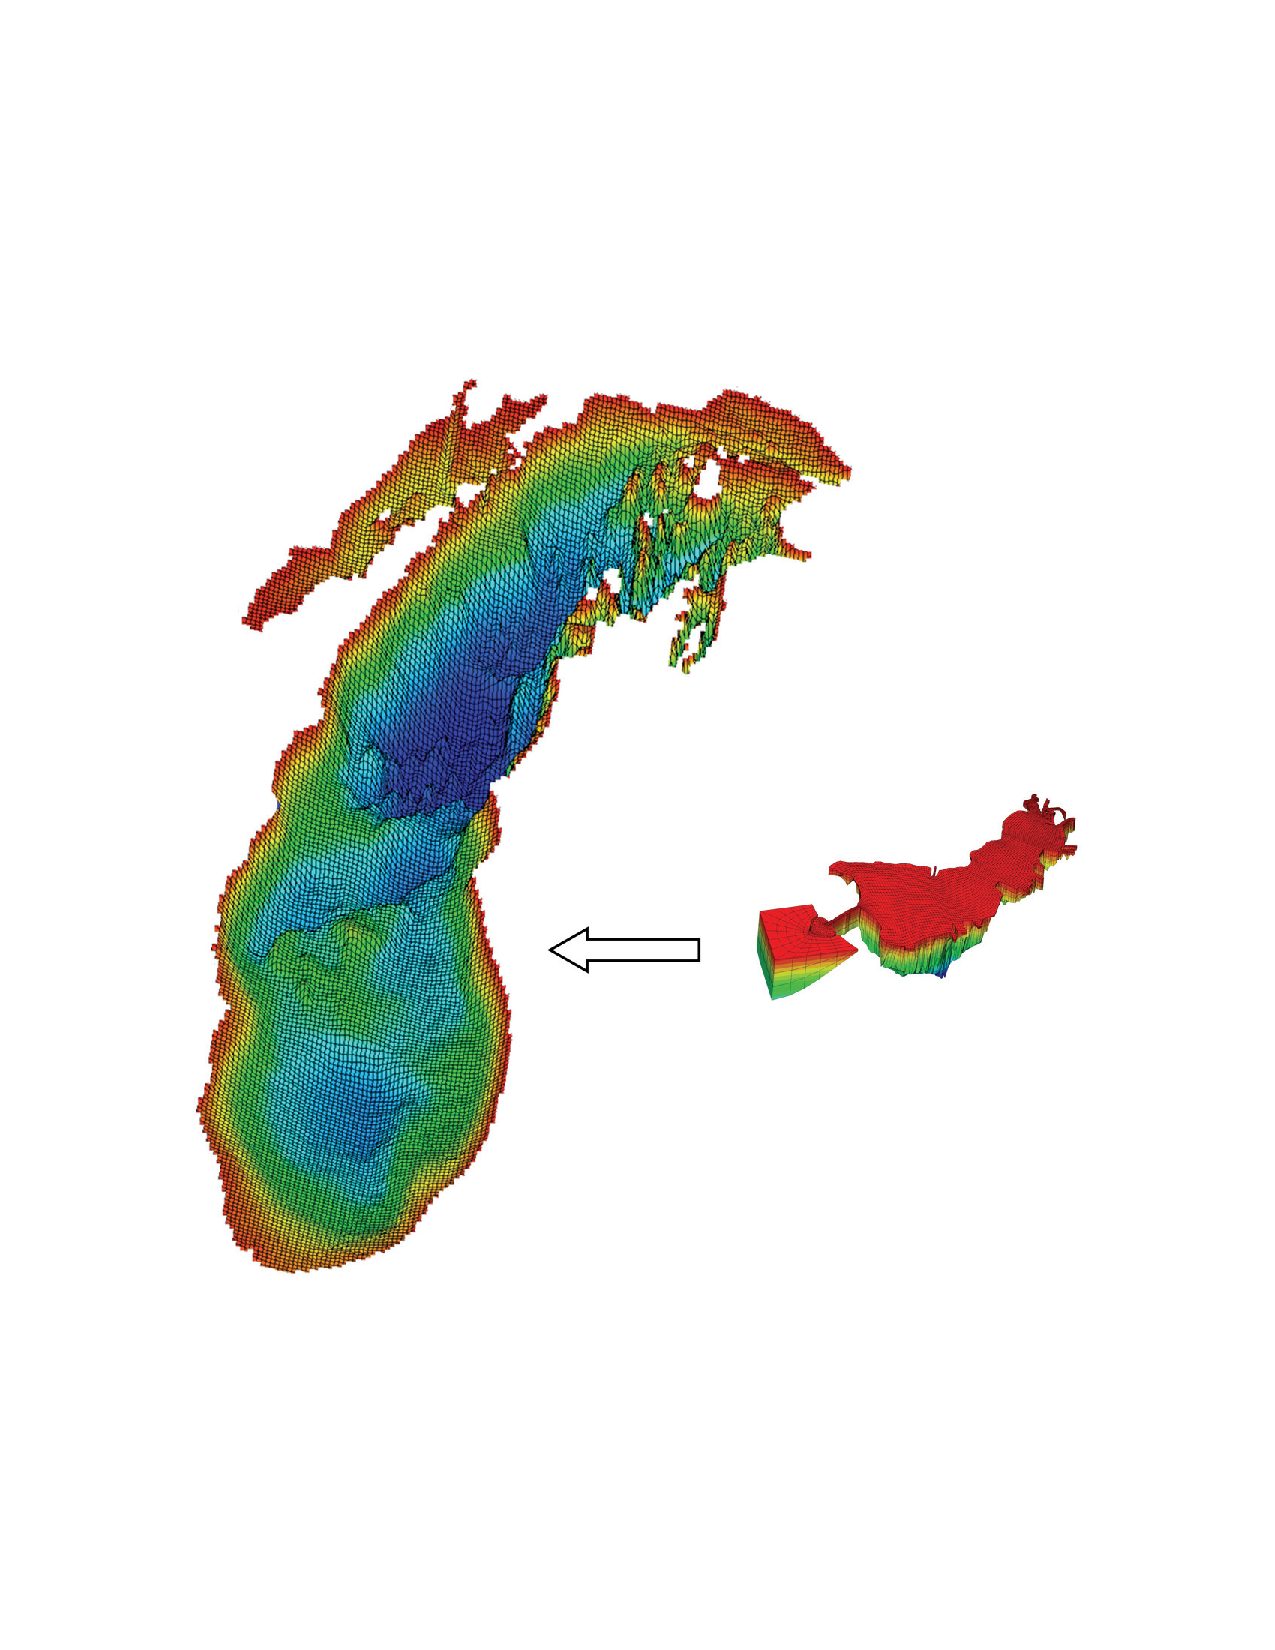
\includegraphics[width=4.3in]{../figures/LakeM+Muskegon.pdf}
\label{fig:LakeM+Muskegon}
\caption{This figure shows the inclusion of the Muskegon Lake into Lake Michigan. The Lake Michigan bathymetry with 2 km grid is from National Oceanic and Atmospheric Administration. http://www.glerl.noaa.gov}
\end{center}
\end{figure}

\normalsize
\subsection{Grid Nesting}

The hydrodynamics of lakes and oceans covers a wide range of spatial and temporal scales. Despite advances in computer technology, modeling full scale phenomena with satisfactory resolution is difficult to achieve in the near future. Therefore, artificial computational boundaries are usually employed in the development of regional numerical models for rivers, estuaries, lakes, or coastal zones. Unrealistic reflecting waves may occur on the computational boundaries where no physical control is present.
Kosloff \cite{Kosloff1986} presented an approach to circumvent the problem by treating the near-boundary region as high dissipating layer; hence waves entering the boundary region are weakened. The concept known as radiation boundary is first
proposed by Sommerfeld \cite{Sommerfeld1949}, which allows the interior wave to pass freely through the artificial boundary with minimum spurious reflection. Orlanski \cite{Orlanski1976} modified the effective phase speed as "floating" phase speed that varies at each time step. Hedley and Yau \cite{Hedley1988} improved the stability by adding constraints on the phase speed. Other efforts to achieve non-reflecting boundary include Engquist and Majda \cite{Engquist1977} and Verboom et al. \cite{Verboom1982}.

Another challenge comes into play when combining different regional numerical models to cover wider area and reduce errors resulted from fictional boundaries. Grid nesting is one of such techniques that increases resolution to simulate small scale phenomena on the area of interest, while large scale circulation is modeled with coarse grid. The above-mentioned non-reflecting boundary methods are aimed at passing out information from inside with minimum disturbances; however, receiving information unhampered from the other side is still an interesting topic. The strategies that handle the information transfer between fine grid mesh (FGM) and coarse grid mesh (CGM) generally fall into two categories: One-way interaction and two-way interaction. In one-way interaction,
boundary conditions of the FGM are imposed from the interpolation of CGM. The FGM boundary values are obtained from the history of CGM; hence CGM computation is independent from the FGM. In two-way interaction, the CGM provides the time-dependant boundary conditions for FGM, followed by the feedback from the FGM: the information from FGM is transferred to CGM where two grids coincident.

The application of grid nesting can be traced back to 1960 when Birchfield predicted hurricane movement, followed by a cyclone model developed by Hill \cite{Hill1967}, a rapidly moving cyclonic model by Wang \cite{Wang1970}, and a typhoon forecast model by Ley and Elsberry \cite{Ley1976}. More recent literature that describes the grid nesting in ocean models includes Spall and Holland \cite{Spall1991}, Fox and Maskell \cite{Fox1995}, and Ginis et al. \cite{Ginis1998}. Zhang et al. \cite{Zhang1986} mentioned that an optimal grid nesting design should have the following properties: (1) all resolvable waves propagate across interfaces smoothly with only minimal changes in amplitude and minimum reflection of energy; (2) mass, momentum and total energy exchanged between the grid systems should be conserved. However, Spall and Holland \cite{Spall1991} and Fox and Maskell \cite{Fox1995} agree that using an interpolation of the CGM variables to obtain the open boundary conditions for the FGM does not have exact conservation at the interface without sacrificing the stability and smoothness of the solution.

As mentioned in Section \ref{chapter:Introduction-ANH}, high-resolution non-hydrostatic modeling in geophysical flows are needed for more accurate weather forecasting and better description of smaller scale phenomena ($<$10 km) \cite{Marshall1997} such as tidal-induced instabilities and wind, buoyancy, or abrupt-bathymetry driven turbulence. However, the research of grid nesting in non-hydrostatic modeling in geophysical flows is still far from being conclusive. This motivated the research of novel domain decomposition methods which are the first step of grid nesting application in non-hydrostatic, geophysical flow modeling. Along the research path, the adjustable non-hydrostatic method, domain decomposition with sequential regularization method, elemental superposition method, and the receding boundary method are developed and documented in this thesis.  